\section{Auswertung}
\label{sec:Auswertung}

%\subsection{Umrechnung der Messdaten} % (fold)
%\label{sec:umrechnung}
Die im Appendix vorliegenden Diagramme lassen zu, Messdaten mit hoher Genauigkeit in ihren Koordinaten zu bestimmen.
Die x-Koordinaten der auszuwertenden Punkte werden in Bezug auf den eingezeichneten Koordinatenursprung bestimmt und für die Auswertung anhand der Gleichung 
\begin{equation}
	U=a_\text{lin}\cdot x+b_\text{lin}
	\label{eq:umrechnung}
\end{equation}
in eine Spannung $U$ umgerechnet.
Die Einheiten von $a_\text{lin}$ und $b_\text{lin}$ sind gemäß der Größenumrechnung passend gewählt, 
es gelten $[a_\text{lin}]=\si{\volt\per\centi\meter}$ und $[b_\text{lin}]=\si{\volt}$.
Diese fehlerbehaftete Umrechnungsparameter stammen von einer linearen Regression mehrer fester Skalenpunkte, für welche die Spannung bekannt ist.
\begin{table}[H]
	\centering
	\sisetup{table-format = -1.3(1)}
		\begin{tabular}{l S S}
		\toprule
		{Plot Nr.}&\multicolumn{2}{c}{Umrechnungsparameter}\\
		&{$a_\text{lin}$/$\:(\si{\volt\per\centi\meter})$} & {$b_\text{lin}$/$\:\si{\volt}$}\\
		\midrule
		\emph{A1}&		0.403(4)& 	-0.12(6)\\
		\emph{A2}&		0.405(4)& 	0.015(6)\\
		\emph{A3}&		2.89(2)& 	-3.9(2)	\\
		\emph{A4}& 		2.40(3)& 	-1.1(5)	\\
		\end{tabular}
	\caption{Umrechnungsparameter der Diagrammlänge zur Spannung. \cite{matplotlib}}
	\label{tab:umrechnung}
\end{table}
\newpage
% section umrechnung (end)
\subsection{Energieverteilung der Elektronen} % (fold)
\label{sec:energiespektren}
Die im Appendix beigefügten Diagramme \emph{A1} und \emph{A2} werden ausgelesen;
das Millimeterpapier lässt eine Genauigkeit von $\SI{1}{\milli\meter}$ zu.
Die Schrittweite entlang der Abzissenachse wird im Allgemeinen so gewählt, dass einerseits \SI{1}{\centi\meter} nicht überschritten wird und 
andererseits ein Unterschied der Werte entlang der Ordinaten-Achse von mindestens $\SI{1}{\milli\meter}$, die größtmögliche Auflösung beim verwandten Papier, gewährleistet ist.
An Stellen mit linearem Verlauf in guter Näherung ist die Schrittweite groß und an Stellen starker Steigungsänderung kleinstmöglich gewählt.
Die eingelesenen Daten sind in Tabellen \ref{tab:E_vert_kalt} und \ref{tab:E_vert_warm} aufgetragen, ihre Darstellung ist in Diagramm \ref{fig:E_vert_kalt} und \ref{fig:E_vert_warm} sichtbar.

\begin{figure}[p]
	\centering
	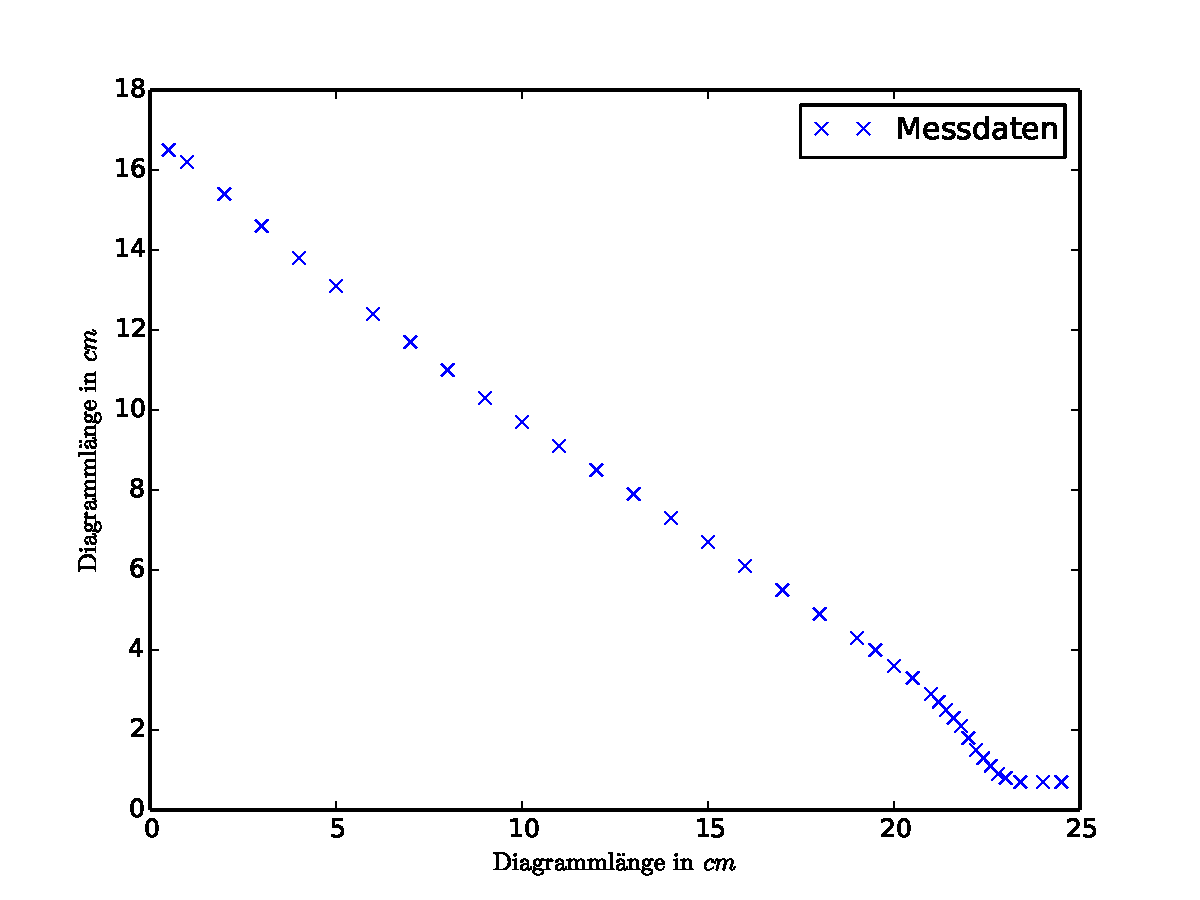
\includegraphics[width=0.8\textwidth]{Bilder/Vert_kalt.pdf}
	\caption{Auftrag der aus Diagramm \emph{A1} entnommenen Daten zum Vergleichen.\cite{matplotlib}}
	\label{fig:E_vert_kalt}
\end{figure}
\begin{figure}[p]
	\centering
	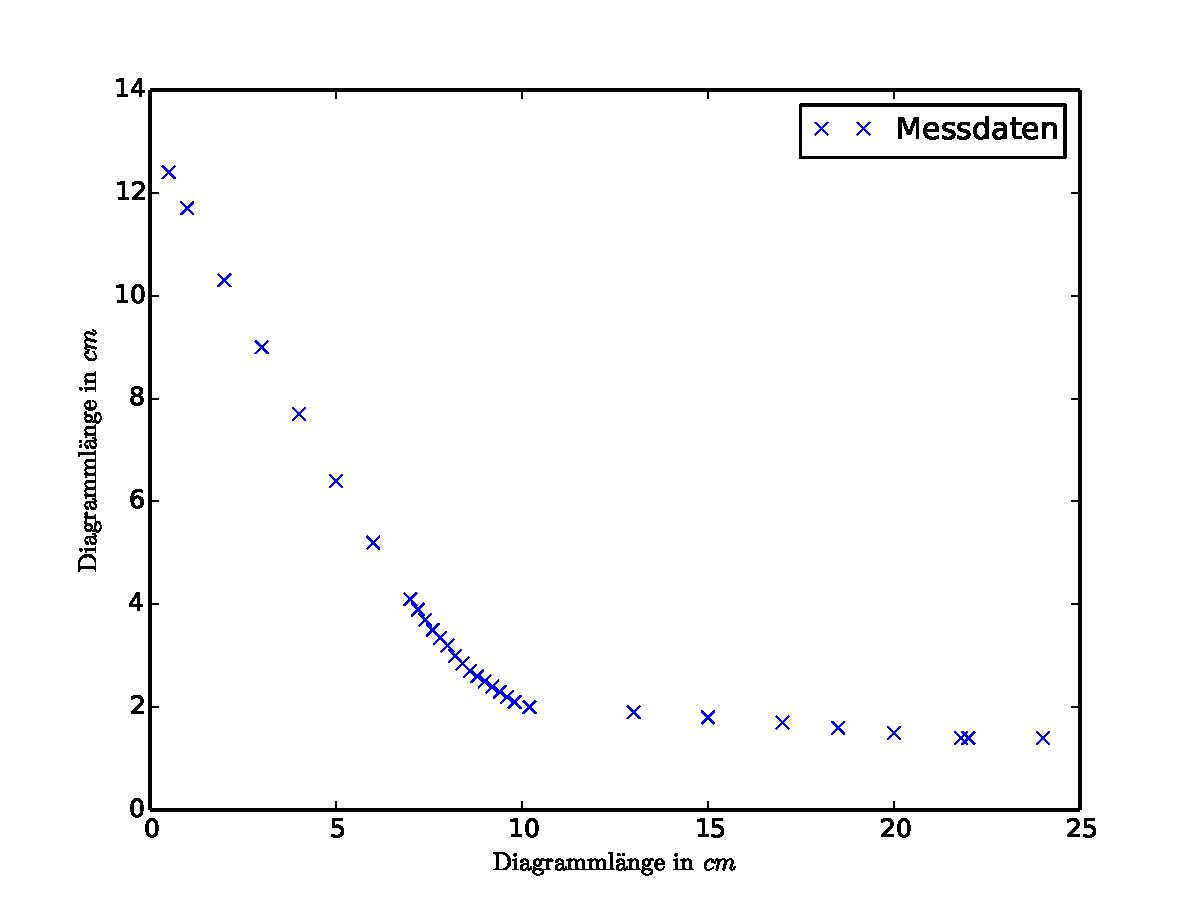
\includegraphics[width=0.8\textwidth]{Bilder/Vert_warm.pdf}
	\caption{Auftrag der aus Diagramm \emph{A2} entnommenen Daten zum Vergleichen.\cite{matplotlib}}
	\label{fig:E_vert_warm}
\end{figure}\begin{figure}[p]
	\centering
	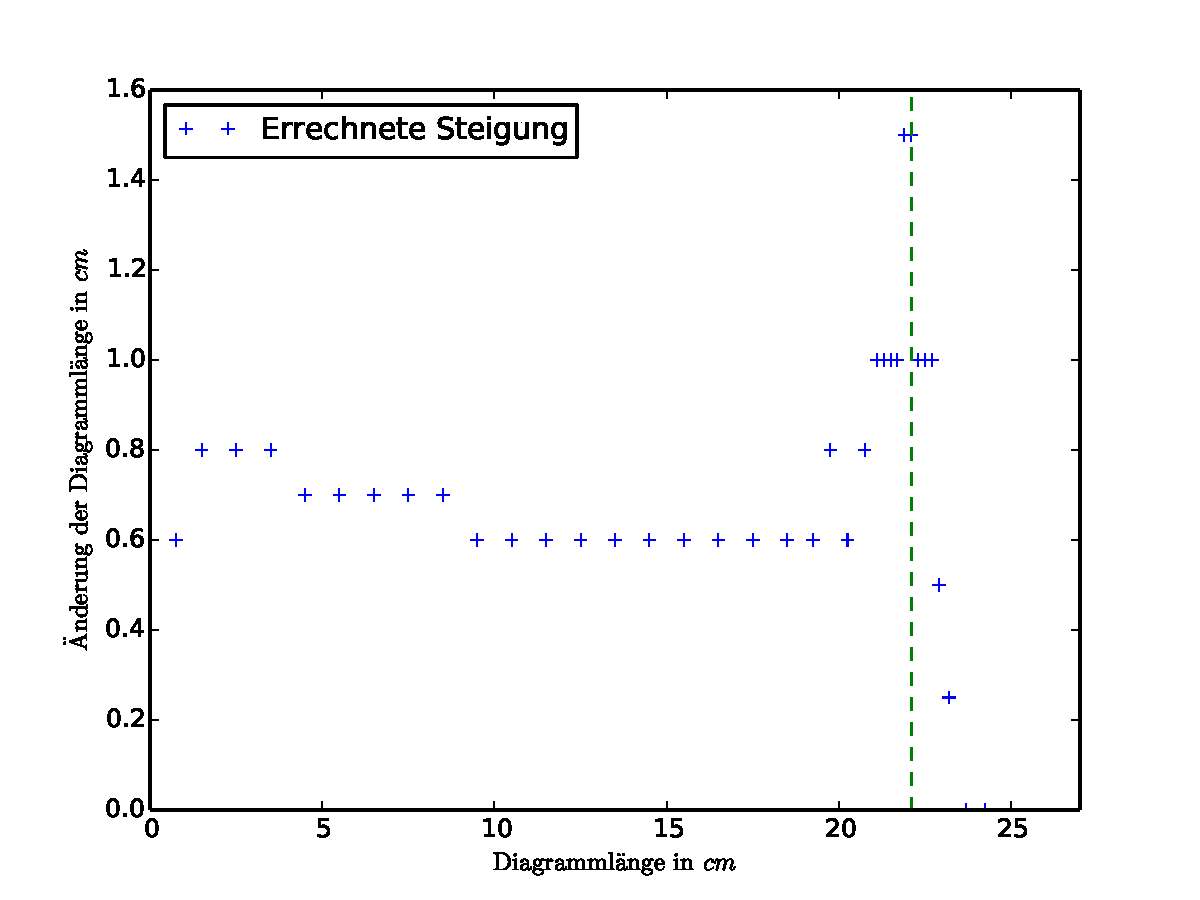
\includegraphics[width=0.8\textwidth]{Bilder/Vert_kalt_diff.pdf}
	\caption{Differentiellen Energieverteilung bei Raumtemperatur.\cite{matplotlib}}
	\label{fig:E_vert_kalt_diff}
\end{figure}
\begin{figure}[p]
	\centering
	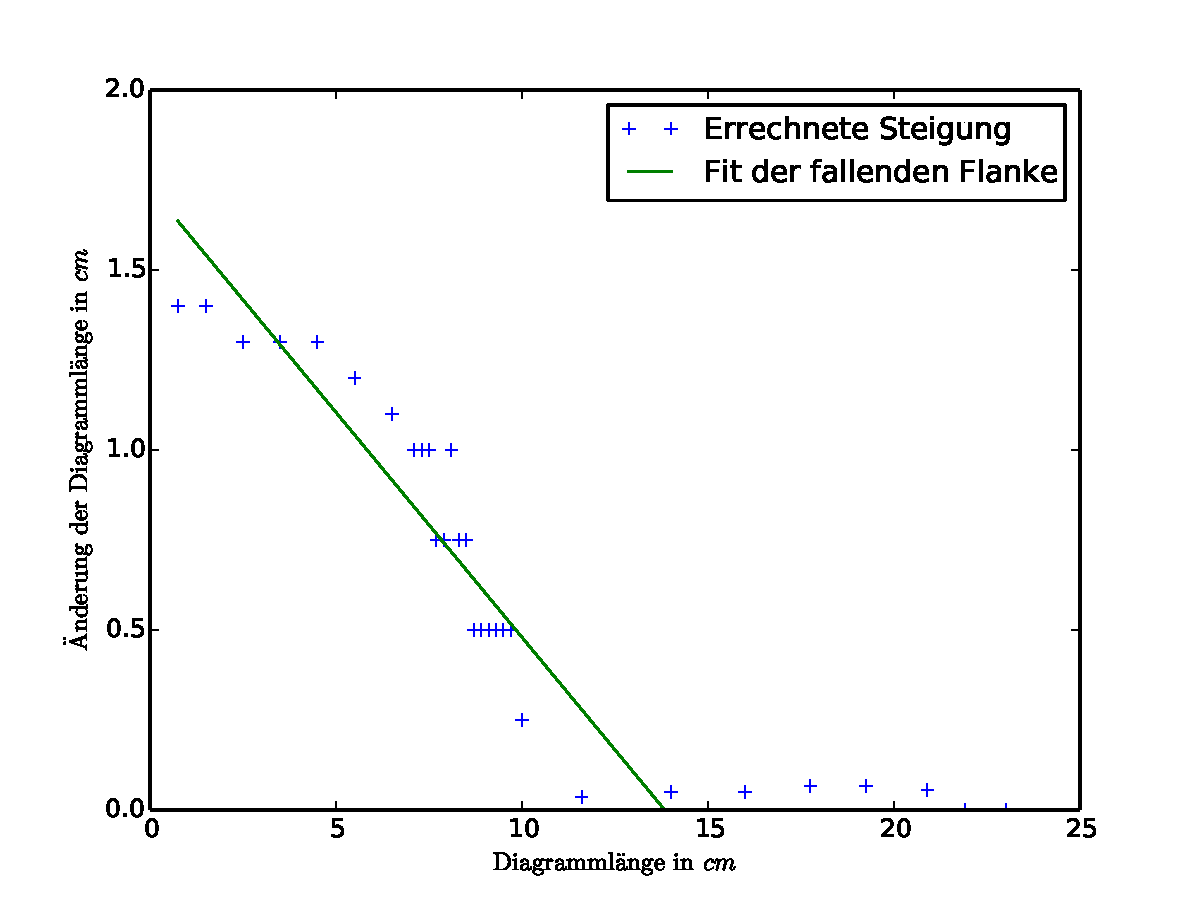
\includegraphics[width=0.8\textwidth]{Bilder/Vert_warm_diff.pdf}
	\caption{Differentiellen Energieverteilung bei erhöhter Temperatur.\cite{matplotlib}}
	\label{fig:E_vert_warm_diff}
\end{figure}
Die aufgenommene integrale Energieverteilung wird in eine differentielle Energieverteilung umgeformt.
Hierzu wird der Abstand zwischen zwei y-Koordinaten durch den Abstand der dazugehörigen x-Koordinaten geteilt und diese Steigung in der Diagramm \ref{fig:E_vert_kalt_diff}, respektive \ref{fig:E_vert_warm_diff}, aufgetragen. 
Diese Steigung wird in die Mitte zwischen den beiden x-Koordinaten gesetzt, damit entspricht das Verfahren einer angenährten Ableitung.

Um das Kontaktpotential $k$ zu bestimmen, wird das Maximum der differentiellen Energieverteilung bei Raumtemperatur bestimmt.
Die Abweichung der Maximalstelle zwischen realer Verteilung und idealer Verteilung, $U=\SI{11}{\volt}$, ist das Kontaktpotential $k$.
Die fallende Flanke der differentiellen Energieverteilung bei erhöhter Temperatur wird linear gefittet.
Hierzu werden die Gleichungen \ref{eq:regress} benützt.

Daher ergeben sich mit der Umrechnungsformel \eqref{eq:umrechnung}
\begin{align}
	x_\text{E.,\SI{26}{\degreeCelsius}}&= \SI{22.1}{\centi\meter}\\
	U_\text{E.,\SI{26}{\degreeCelsius}}&= \SI{8.8(1)}{\volt}\\
	k_\text{\SI{26}{\degreeCelsius}} &= \SI{2.2(1)}{\volt}
	\label{qu:k1}
\end{align}
\begin{align}
	x_\text{E.,\SI{120}{\degreeCelsius}}&= \SI{14(2)}{\centi\meter}\\
	U_\text{E.,\SI{120}{\degreeCelsius}}&= \SI{5.6(6)}{\volt}\\
	k_\text{E.,\SI{120}{\degreeCelsius}}&= \SI{5.4(6)}{\volt}
\end{align}

\begin{table}
	\centering
	\sisetup{table-format=2.1}
	\begin{tabular}{S S}
		\toprule
		\multicolumn{2}{c}{Abgelesene Koordinaten der Messkurve}\\
		{Koordinate x/\si{\centi\meter}}&{Koordinate y/\si{\centi\meter}}\\
		\midrule
			00.5&	16.5\\
			01.0&	16.2\\
			02.0&	15.4\\
			03.0&	14.6\\
			04.0&	13.8\\
			05.0&	13.1\\
			06.0&	12.4\\
			07.0&	11.7\\
			08.0&	11.0\\
			09.0&	10.3\\
			10.0&	09.7\\
			11.0&	09.1\\
			12.0&	08.5\\
			13.0&	07.9\\
			14.0&	07.3\\
			15.0&	06.7\\
			16.0&	06.1\\
			17.0&	05.5\\
			18.0&	04.9\\
			19.0&	04.3\\
			19.5&	04.0\\
			20.0&	03.6\\
			20.5&	03.3\\
			21.0&	02.9\\
			21.2&	02.7\\
			21.4&	02.5\\
			21.6&	02.3\\
			21.8&	02.1\\
			22.0&	01.8\\
			22.2&	01.5\\
			22.4&	01.3\\
			22.6&	01.1\\
			22.8&	00.9\\
			23.0&	00.8\\
			23.4&	00.7\\
			24.0&	00.7\\
			24.5&	00.7\\
		\bottomrule
	\end{tabular}
	\caption{Ausgelesene Daten der Messkurve \emph{A1}: Energieverteilung bei Raumtemperatur}
	\label{tab:E_vert_kalt}
\end{table}
\begin{table}[p]
	\centering
	\sisetup{table-format=2.1}
	\begin{tabular}{S S}
		\toprule
		\multicolumn{2}{c}{Abgelesene Koordinaten der Messkurve}\\
		{Koordinate x/\si{\centi\meter}}&{Koordinate y/\si{\centi\meter}}\\
		\midrule
		00.5&	12.4\\
		01.0&	11.7\\
		02.0&	10.3\\
		03.0&	09.0\\
		04.0&	07.7\\
		05.0&	06.4\\
		06.0&	05.2\\
		07.0&	04.1\\
		07.2&	03.9\\
		07.4&	03.7\\
		07.6&	03.5\\
		07.8&	03.3\\
		08.0&	03.2\\
		08.2&	03.0\\
		08.4&	02.8\\
		08.6&	02.7\\
		08.8&	02.6\\
		09.0&	02.5\\
		09.2&	02.4\\
		09.4&	02.3\\
		09.6&	02.2\\
		09.8&	02.1\\
		10.2&	02.0\\
		13.0&	01.9\\
		15.0&	01.8\\
		17.0&	01.7\\
		18.5&	01.6\\
		20.0&	01.5\\
		21.8&	01.4\\
		22.0&	01.4\\
		24.0&	01.4\\
		\bottomrule
	\end{tabular}
	\caption{Ausgelesene Daten der Messkurve \emph{A2}: Energieverteilung bei erhöhter Temperatur}
	\label{tab:E_vert_warm}
\end{table}

Für die folgende Auswertung wird nur das Kontaktpotential $k$ aus der Messung bei $\SI{26}{\degreeCelsius}$ betrachtet.
Die Unterschiede in den Kontaktpotentialen zu verschiedenen Temperaturen wird in Abschnitt \ref{sec:disk_temp} diskutiert.
% section aufnahme_der_energiespektren (end)




\subsection{Franck--Hertz-Kurven} % (fold)
\label{sec:fhk}
Das im Anhang beigefügte Diagramm \emph{A4} zeigt die Franck--Hertz-Kurve der benutzen Apparatur.
Die x-Koordinaten der lokalen Maxima sind in Tabelle \ref{tab:fhkurve} aufgetragen.
\begin{table}
	\centering
	\sisetup{table-format = -2.1}
		\begin{tabular}{S}
		\toprule
		{$x_\text{Max}$/$\:(\si{\centi\meter})$}\\
		\midrule
			05.2\\
			07.2\\
			09.3\\
			11.3\\
			13.4\\
			15.6\\
			17.8
		\end{tabular}
	\caption{x-Koordinaten der Maxima der Franck--Hertz-Kurve, ausgelesen aus Appendix \emph{A4}.}
	\label{tab:fhkurve}
\end{table}
Bei der Betrachtung der Abstände zwischen den Maxima ergibt sich ein umgerechneter Wert von
\begin{equation}
	U=\SI{3.9(5)}{\volt}.
\end{equation}
Diese Spannung entspricht der Beschleunigungspannung, die bei der Franck--Hertz-Röhre zur Anregung des Quecksilbers zum ersten Energieniveau benötigt wird.

Bei Erreichen dieser Spannung, respektive dieser kinetischen Energie, sind inelastische Stöße möglich; die Elektronen geben beim Zusammenstoß Energie zur Anregung an Quecksilber.
Der Auffängeranodenstrom $I$ ist ein Maß für die Anzahl der Elektronen, die nach eventuellen Stößen mit Quecksilber und nach Erreichen der Beschleunigungsanode ausreichende kinetische Energie aufweisen, um das Gegenfeld zu überwinden.
Ein Abfallen des Stromes deutet auf auftretenden Mangel an kinetischer Energie hin.\\
Der Energieverlust der Elektronen durch elastische Stöße wird nicht berücksichtigt, da dies im Vergleich zum Energieverlust durch inelastische Stöße geringen Effekt auf die Stromstärke hat und im Kontrast zum inelastischen Stoß nicht ausschließlich an ausgezeichneten Spannungen stattfindet.

Aus dem ermittelten Wert $U$ ergeben sich die weiteren Größen erste Anregungsenergie $E_\text{Hg, 1}$, Anregungsfrequenz $f_\text{Anregung}$ und Wellenlänge der emittierten Strahlung $\lambda$.
\begin{align}	
	E_\text{Hg}		&=\SI{6.3(7)e-19}{\joule}\\
	f_\text{Anregung}	&=\SI{10(1)e+14}{\hertz}\\
	\lambda				&=\SI{320(40)}{\nano\meter}
\end{align}
Dieses Messergebnis für die erste Anregungsenergie $E_\text{Hg}$ weicht von der Literaturangabe, $E_\text{Hg,Lit.}=\SI{4.9}{\electronvolt}$ \cite{IonEx}, um $20.4\%$ ab.

Das Kontaktpotential $k$ ist abschätzbar durch die globale Verschiebung der Maxima.
Die Maximalstellen sind im idealen Verlauf Vielfache der Anregungsenergie $E_\text{Hg, 1}$, 
die Abweichungen der realen Stellen von der Theorie ist das Kontaktpotential $k$.
Es wird das Kontaktpotential
\begin{equation}
	k=\SI{3.5(10)}{\volt}
	\label{qu:k2}
\end{equation}
ermittelt.

% section franck_hertz_kurven (end)

\subsection{Ionisierungskurven von Quecksilber} % (fold)
\label{sec:ion}
Das im Anhang angefügte Diagramm \emph{A3} zeigt die Ionisierungskurve von Quecksilber.
Die Messdaten werden wie in Abschnitt \ref{sec:energiespektren} aufgenommen, 
die Daten sind in Tabelle \ref{tab:ion} aufgetragen.

\begin{table}[p]
	\centering
	\sisetup{table-format=2.1}
	\begin{tabular}{S S}
		\toprule
		\multicolumn{2}{c}{Abgelesene Koordinaten}\\
		{Koordinate x/\si{\centi\meter}}&{Koordinate y/\si{\centi\meter}}\\
		\midrule
			01.5&	02.6\\
			02.0&	02.6\\
			03.0&	02.6\\
			04.0&	02.6\\
			05.0&	02.6\\
			05.3&	02.6\\
			05.4&	02.7\\
			05.5&	02.9\\
			05.6&	03.3\\
			05.7&	04.0\\
			05.8&	04.6\\
			05.9&	06.0\\
			06.0&	07.0\\
			06.1&	08.8\\
			06.2&	10.0\\
			06.3&	11.8\\
			06.4&	14.0\\
			06.5&	15.6\\
			06.6&	17.2\\
			06.7&	17.2\\
			06.8&	17.2\\
			07.0&	17.2\\
			08.0&	17.2\\
			09.0&	17.2\\
			10.0&	17.2\\
			11.0&	17.2\\
			12.0&	17.2\\
			13.0&	17.2\\
			14.0&	17.2\\
			15.0&	17.2\\
			16.0&	17.2\\
			17.0&	17.2\\
			18.0&	17.2\\
			19.0&	17.2\\
			20.0&	17.2\\
			21.0&	17.2\\
			22.0&	17.2\\
		\bottomrule
	\end{tabular}
	\caption{Ausgelesene Daten der Messkurve \emph{A3}: Ionisierungskurve von Quecksilber}
	\label{tab:ion}
\end{table}

Über eine lineare Regression \eqref{eq:regress} wird ein Fit an die steigende Flanke gelegt und dessen Nullstelle bestimmt.
Dabei ist zu berücksichtigen, dass die Nullstelle des in Abbildung \ref{fig:ion} gezeigten Verlaufes von der Nullstelle der tatsächlichen Ionisierungskurve abweicht, da in Abbildung \ref{fig:ion} wie in Tabelle \ref{tab:ion} die Koordinaten der Kurve aufgetragen sind.
Zur Bestimmung der gewünschten Nullstelle wird der x-Wert des Fits in vorliegenden Koordinaten bei $y=\SI{2.6}{\centi\meter}$, dem Nullwert der Ionisierungskurve in dieser Darstellung, bestimmt.
Die Nullstelle der Ionisierungskurve hat die x-Koordinate% und umgerechnete Spannung
\begin{equation}
	x_\text{Ion}=\SI{5.5(5)}{\centi\meter}
	\label{qu:ion}
\end{equation}
Für die Spannung $U_\text{Ion}$, die zur Ionisierung von Quecksilber anliegen muss, gilt im Weiteren
\begin{equation}
	\tilde{U}_\text{Ion}=U_\text{Ion}+k
\end{equation}
mit der in der Auswertung bestimmten Spannung $\tilde{U}_\text{Ion}$, die sich aus der Umrechnung von der Nullstelle \ref{qu:ion} ergibt.
Mit dem Mittelwert der in Abschnitt \ref{sec:energiespektren}, Gl. \eqref{qu:k1} und \ref{sec:fhk}, Gl. \eqref{qu:k2} gefundenen Kontaktpotentiale $k$,
\begin{equation}
	k=\SI{2.9(5)}{\volt},
\end{equation}
ergießt sich für die Ionisierungsenergie der Wert
\begin{equation}
	E_\text{Hg, Ion}=\SI{9.1(16)}{\electronvolt}.
\end{equation}
Dieses Messergebnis weicht von der Literaturangabe, $E_\text{Hg, Ion}=\SI{10.44}{\electronvolt}$ \cite{IonHg}, um $12.8\%$ ab, 
der Literaturwert liegt im Bereich der Standardabweichung des Messergebnisses.
\begin{figure}[H]
	\centering
	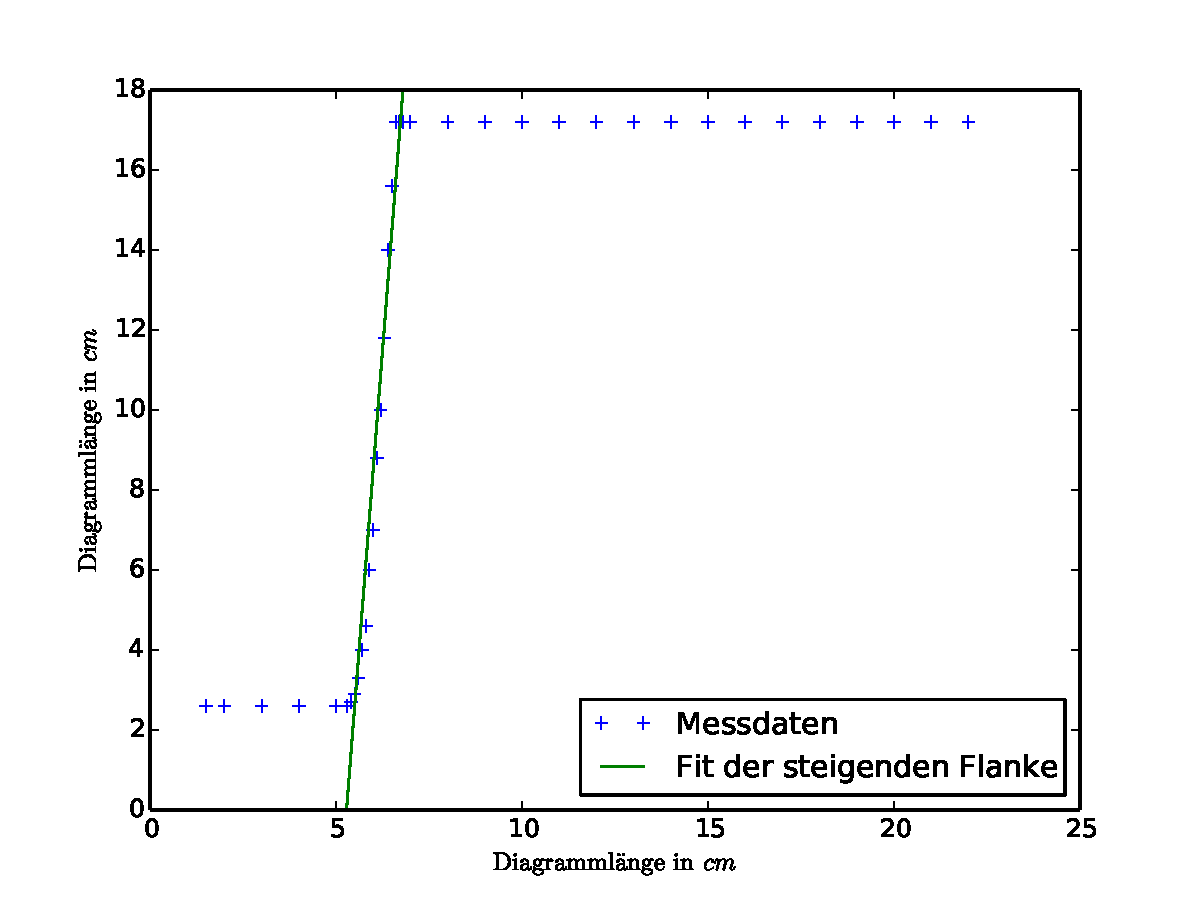
\includegraphics[width=0.75\textwidth]{Bilder/Vert_ion.pdf}
	\caption{Auftrag der aus Diagramm \emph{A3} entnommenen Daten mit Regression der steigenden Flanke. \cite{matplotlib}}
	\label{fig:ion}
\end{figure}
% section ion (end)

